\documentclass[border=12pt]{standalone}
\def\pgfsysdriver{pgfsys-dvisvgm.def}
\usepackage[dvisvgm]{xcolor}
\usepackage{xeCJK}
\setCJKmainfont{HaranoAjiGothic-Regular.otf}[BoldFont=HaranoAjiGothic-Bold.otf]
\setCJKsansfont{HaranoAjiGothic-Regular.otf}[BoldFont=HaranoAjiGothic-Bold.otf]
\usepackage{amsmath,amssymb,tikz,lmodern}
\usetikzlibrary{arrows.meta,positioning,calc,fit,backgrounds}
\renewcommand{\familydefault}{\sfdefault}
\definecolor{ink}{HTML}{25322F}
\definecolor{green}{HTML}{246657}
\definecolor{tint}{HTML}{EEF4F0}
\definecolor{soft}{HTML}{C6D2CC}
\definecolor{muted}{HTML}{52615B}
\newif\ifJapanese
\newcommand{\Tx}[2]{\ifJapanese #1\else #2\fi}
\newcommand{\Eff}{\overline{\operatorname{Eff}}}
\newcommand{\heading}[3]{{\color{green}\bfseries #1\quad\Tx{#2}{#3}}\\[5pt]}
% A white rectangle makes the complete citation label clickable, including spaces.
\newcommand{\refurl}[2]{\special{dvisvgm:raw <a xlink:href="#1" target="_blank" rel="noopener noreferrer">}{\setlength{\fboxsep}{0pt}\colorbox{white}{\color{green}\underline{\strut #2}}}\special{dvisvgm:raw </a>}}
\newcommand{\refedge}[3]{\refurl{\csname source#1\endcsname\string##page=#2}{#3}}
\newcommand{\SF}[2]{\refedge{sf}{#1}{#2}}
% GitHub's file preview does not support PDF page fragments.
\newcommand{\LA}[2]{\refurl{\sourcela}{#2}}
\newcommand{\Sch}[2]{\refedge{sch}{#1}{#2}}
\newcommand{\PS}[2]{\refedge{ps}{#1}{#2}}
\tikzset{
 card/.style={draw=soft,fill=white,rounded corners=2pt,align=left,text=ink,font=\fontsize{10.5}{14}\selectfont,inner xsep=12pt,inner ysep=10pt,text width=14.4cm},
 half/.style={card,text width=6.45cm,minimum height=2.05cm},
 result/.style={card,draw=green,fill=tint,line width=.9pt},
 reason/.style={align=left,text=muted,font=\fontsize{9}{12}\selectfont,inner sep=0pt,text width=12.7cm},
 branchreason/.style={reason,text width=5.95cm},
 edge/.style={-{Stealth[length=2.4mm]},draw=green,line width=1pt},
 wire/.style={draw=green,line width=1pt},
}
% Keep the arrow in a dedicated left gutter; explanations never cover it.
\newcommand{\flow}[3]{
 \coordinate (#2-from) at ($(#1.south)+(-6.9,0)$);
 \coordinate (#2-to) at ($(#2.north)+(-6.9,0)$);
 \draw[edge] (#2-from)--(#2-to);
 \node[reason,anchor=west] (#2-reason) at ($(#2-from)!.5!(#2-to)+(.55,0)$) {#3};
}


\newcommand{\CiteSource}[2]{\refurl{\csname source#1\endcsname}{#2}}

\expandafter\def\csname sourceS\endcsname{https://github.com/openai/math/blob/adc7f1241b42e322a6451854ab7e4b4c146bf78a/preprints/Lifting-sections-from-the-reduced-support-of-an-adjoint-September-27-2026/paper.pdf}
\expandafter\def\csname sourceNV\endcsname{https://github.com/openai/math/blob/adc7f1241b42e322a6451854ab7e4b4c146bf78a/preprints/Fourfold-nonvanishing-by-minimal-metrics-and-moving-jets-September-27-2026/paper.pdf}
\expandafter\def\csname sourceFG\endcsname{https://www.math.kyoto-u.ac.jp/~fujino/fg-comp-final.pdf}
\expandafter\def\csname sourceKS\endcsname{https://people.math.harvard.edu/~mpopa/papers/oxford.pdf}
\expandafter\def\csname sourceHash\endcsname{https://arxiv.org/html/1609.00121v4}
\expandafter\def\csname sourceBir\endcsname{https://arxiv.org/pdf/0706.1792}
\expandafter\def\csname sourceSaito\endcsname{https://doi.org/10.2977/PRIMS/1195171082}
\expandafter\def\csname sourceUfour\endcsname{https://github.com/openai/math/blob/adc7f1241b42e322a6451854ab7e4b4c146bf78a/preprints/Uniform-effective-log-Iitaka-fibrations-for-fourfolds-September-26-2026/paper.pdf}

\Japanesefalse
\begin{document}
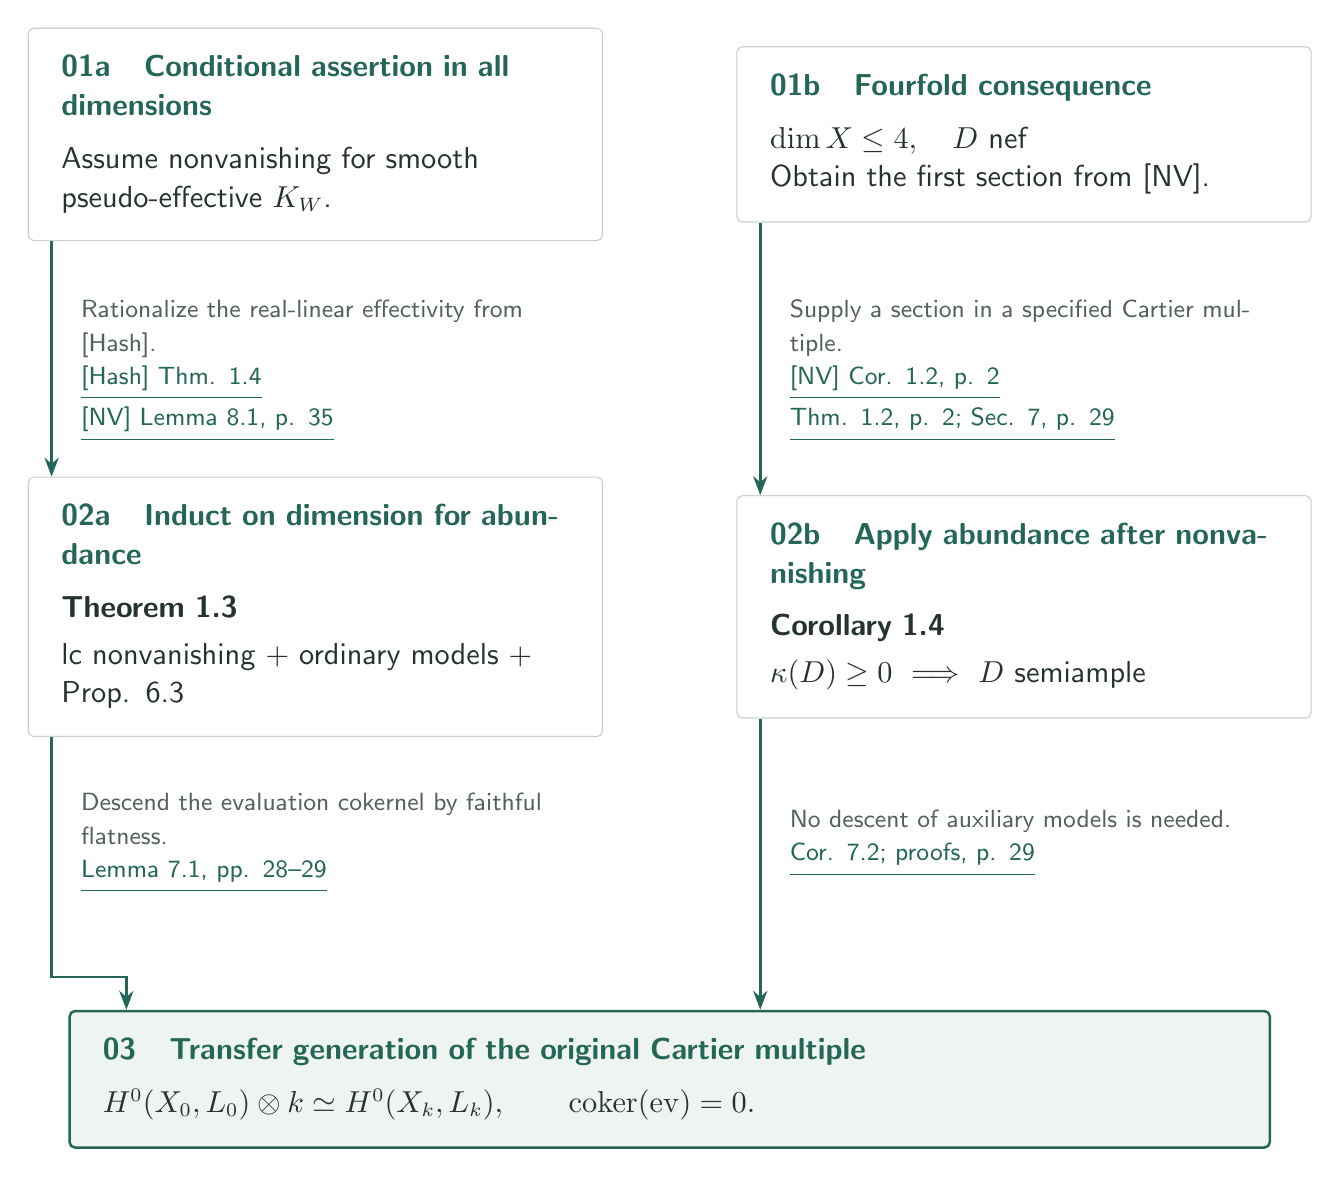
\begin{tikzpicture}
\node[half] (all) at (-4.5,0) {\heading{01a}{全次元の条件付き命題}{Conditional assertion in all dimensions}\Tx{滑らかな擬有効 $K_W$ の非消滅を仮定する。}{Assume nonvanishing for smooth pseudo-effective $K_W$.}};
\node[half] (four) at (4.5,0) {\heading{01b}{四次元の帰結}{Fourfold consequence}$\dim X\le4,\quad D\ \text{nef}$\\\Tx{[NV] から最初の切断を得る。}{Obtain the first section from [NV].}};
\node[half] (allout) at (-4.5,-6) {\heading{02a}{次元帰納法で豊富性へ}{Induct on dimension for abundance}\textbf{Theorem 1.3}\\[3pt]\Tx{lc 非消滅＋通常のモデル＋Prop. 6.3}{lc nonvanishing + ordinary models + Prop. 6.3}};
\node[half] (fourout) at (4.5,-6) {\heading{02b}{非消滅後の豊富性を適用する}{Apply abundance after nonvanishing}\textbf{Corollary 1.4}\\[3pt]$\kappa(D)\ge0\ \Longrightarrow\ D\ \text{semiample}$};
\node[result] (base) at (0,-12) {\heading{03}{元の Cartier 倍の生成性を体の間で移す}{Transfer generation of the original Cartier multiple}$H^0(X_0,L_0)\otimes k\simeq H^0(X_k,L_k),\qquad\operatorname{coker}(\mathrm{ev})=0.$};
\draw[edge] ($(all.south)+(-3.35,0)$)--($(allout.north)+(-3.35,0)$);
\node[branchreason] at (-4.5,-3) {\Tx{[Hash] の実線形有効性を有理化する。}{Rationalize the real-linear effectivity from [Hash].}\\\CiteSource{Hash}{[Hash] Thm. 1.4}\\\CiteSource{NV}{[NV] Lemma 8.1, p. 35}};
\draw[edge] ($(four.south)+(-3.35,0)$)--($(fourout.north)+(-3.35,0)$);
\node[branchreason] at (4.5,-3) {\Tx{指定 Cartier 倍に非零切断を供給。}{Supply a section in a specified Cartier multiple.}\\\CiteSource{NV}{[NV] Cor. 1.2, p. 2}\\\CiteSource{S}{Thm. 1.2, p. 2; Sec. 7, p. 29}};
\draw[edge] ($(allout.south)+(-3.35,0)$)--(-7.85,-10.7)--(-6.9,-10.7)--($(base.north)+(-6.9,0)$);
\draw[edge] ($(fourout.south)+(-3.35,0)$)--($(base.north)+(1.15,0)$);
\node[branchreason] at (-4.5,-9) {\Tx{評価写像の余核を忠実平坦性で降ろす。}{Descend the evaluation cokernel by faithful flatness.}\\\CiteSource{S}{Lemma 7.1, pp. 28--29}};
\node[branchreason] at (4.5,-9) {\Tx{補助モデルの降下は不要。}{No descent of auxiliary models is needed.}\\\CiteSource{S}{Cor. 7.2; proofs, p. 29}};
\end{tikzpicture}
\end{document}
